%-----------------------------------------------------------------------------------------------
\chapter{Marker recognition}\label{sect:markerRec}
%-----------------------------------------------------------------------------------------------

In this chapter there will be a summary of the image processing algorithms tried and used for the recognition of the fiducial markers.
From a computer vision point of view the task is to detect joint line segments.
This is a relatively easy task in image processing, there are many well tried algorithms for it.

In this chapter will be a short summary of the algorithms used for testing and performance comparison.
The preprocessing steps used for preparing the images for the line fitters (segmentation, thresholding, filtering etc.) will also be discussed.

The general flow of processing is the same for every line fitting solution.
The input is the raw image taken\footnote{In the development phase there were rendered pictures used for better repeatability} by the observer.
The first problem is finding the RQIM on the picture.
When the marker area is located, it is necessary to discard the only partially visible and/or unrecognisable quads.
At this point there is an image or set of images containing potentially good quads.
The process here diverges depending on which line fitting algorithm is used.
They all need differently conditioned input images for optimal performance.
The line fitter routines not necessarily have the same output format\footnote{Some return line segments defined by their endpoint, others use the polar representation of a lin, etc.}, so conversion may be needed.
This is the end of the marker recognition phase.
This step of the process takes the raw input image and initiates quad structures based on the observed picture.

Four separate line fitters are profiled in this experiment.
\begin{itemize}
	\item Hough-transformation
	\item Corner detection
	\item Skeletoning detector
	\item Gradient detector (enhanced Hough transformation)
\end{itemize}
The first one uses the classic Hough-transformation for line detection.
In the OpenCV framework there is another, probabilistic implementation of the transformation.
It will also be tested.

The second detector is based on corner recognition.
There are more variants of this method to try out, too.
The corner metrics of a feature can be calculated differently with (Harris metric, eigenvalues, etc.) varying results.
It is also needed for the solution to be scale invariant, which also can be achieved in a number of ways.

The third alternative uses skeletoning for line detection.
It is a RANSAC-like method, which makes it very robust, though quite computationally expensive.
The core concept is to thin the observed marker (band) down to single pixel lines and try to find two point with the most inliers.

The gradient detector is a bit Hough-like in it's nature.
It uses the image gradient to calculate the angle in the Hough-space, and the pixels only vote in their distance parameter.

A typical marker shot with partial visibility is shown figure \figref{partialMarkerShot}.
\begin{figure}[ht]
	\centering
	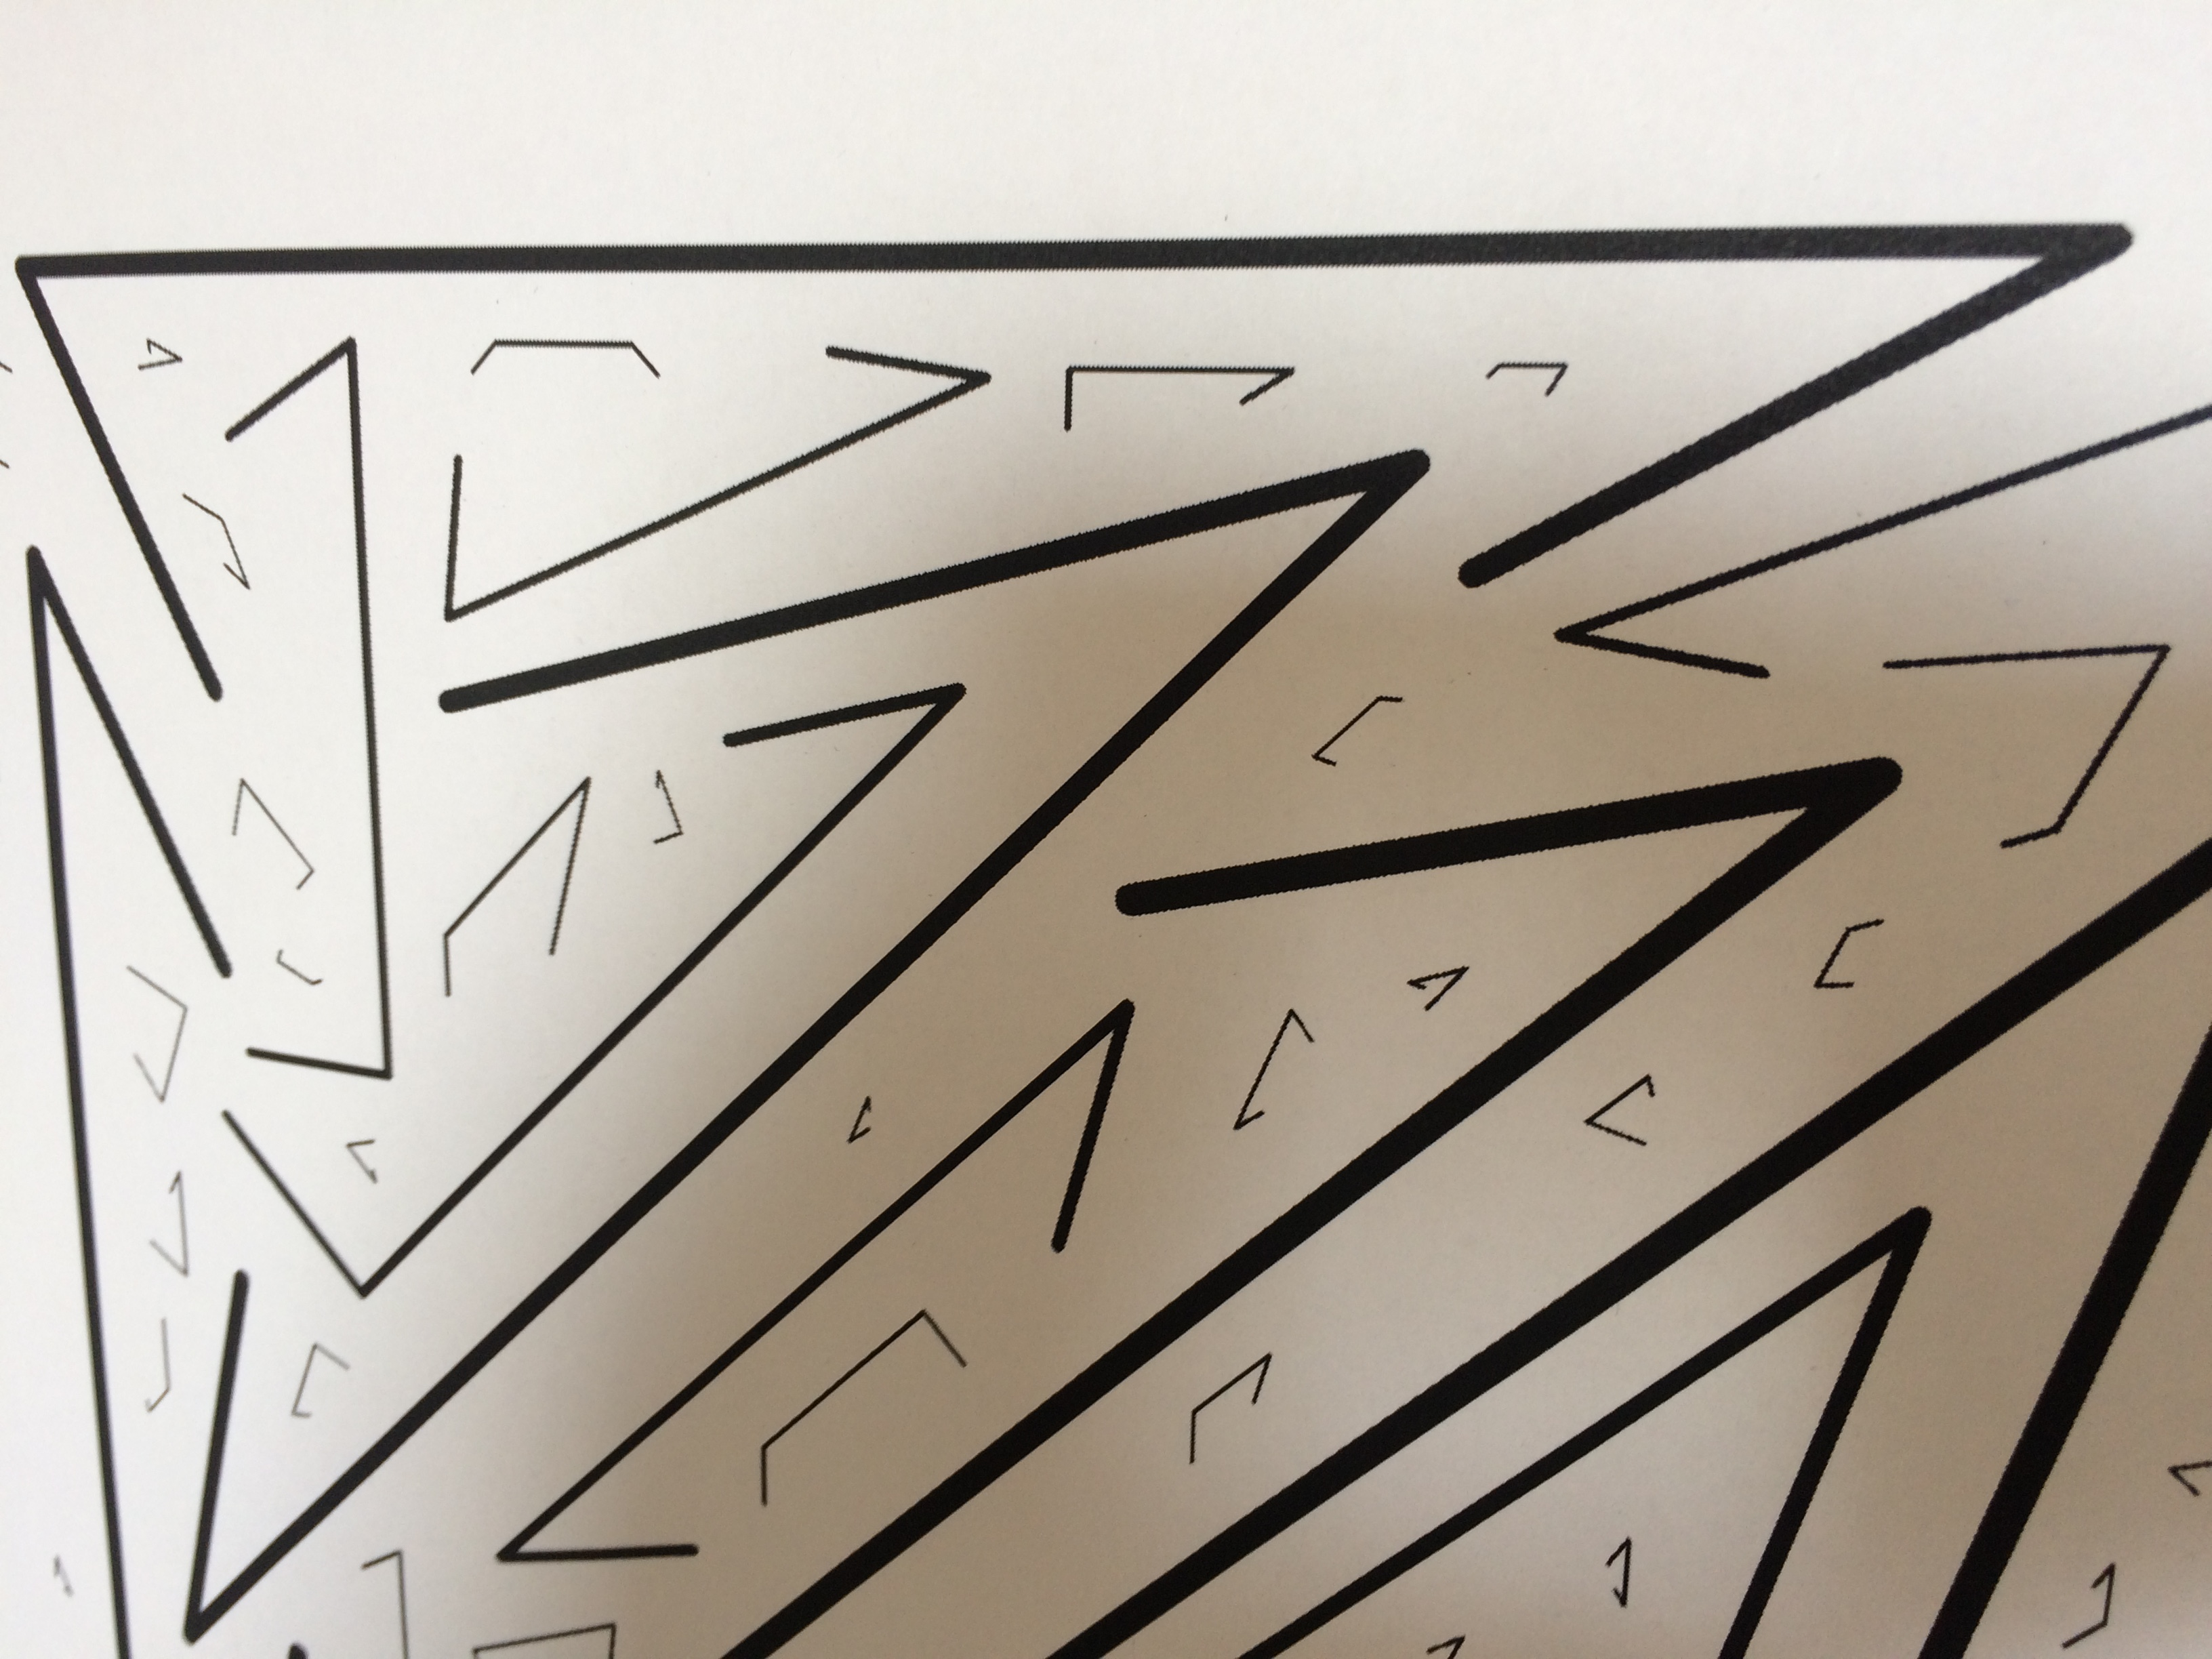
\includegraphics[width=0.75\textwidth]{figures/t35_01.JPG}
	\caption{Partially visible marker (taken with commercial smartphone)}
	\label{fig:partialMarkerShot}
\end{figure}

%-----------------------------------------------------------------------------------------------
\section{Preprocessing}
%-----------------------------------------------------------------------------------------------

The preprocessing is done in two stages.
The first is the segmentation, when quad-like blobs are found.
The second step is the preparation of the aforementioned blobs for the line fitting algorithms' needs.

%-----------------------------------------------------------------------------------------------
\subsection{Segmentation}
%-----------------------------------------------------------------------------------------------

The segmentation process is carried out on images roughly like the one shown in figure \figref{partialMarkerShot}.
First the photos are converted to binary format by applying a threshold.
The image is inverted in the process, because it makes more sense for the objects to be marked with non-zero elements than vice-versa.
The threshold's value is determined using Otsu's method, which maximises the inter-class variance of the clusters\footnote{Foreground and background}.
The implementation is provided by the OpenCV framework.

Afterwards, the binary image is conditioned with a \emph{close} morphology operator.
The closing removes the gaps from the large connected areas (possible quads) and removes the \emph{salt and pepper}-like noise.
In the current implementation the kernel size of the morphology operator is constant, however it could be beneficial to calculate it from the global or local image parameters\footnote{e.g. image size, area of the connected region, etc.}.

The segmentation is based on finding continuous contours on the binary image.
The OpenCV framework provides great functionality for this.
The implementation is based on calculating the 8-neighbour chain code for the binary blobs on the image.
The functions returns a list of list of points for the borders os each distinct contour.

The next step is the filtering of the found blobs.
First the surely partial quads are discarded.
This is done by calculating the bounding box of the contours, and if one of it's sides are touching the image border, the blob is marked as partial.
With this approach it is possible that some fully visible quads that only touch the image border with one of their corner are lost.
This problem can be easily fixed by checking the neighbourhood of the contact point, but this is not yet implemented.

\begin{figure}[ht]
	\begin{subfigure}{0.3\textwidth}
		\centering
		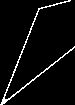
\includegraphics{figures/quad3.png}
	\end{subfigure}
	\begin{subfigure}{0.3\textwidth}
		\centering
		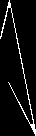
\includegraphics{figures/quad4.png}
	\end{subfigure}
	\begin{subfigure}{0.3\textwidth}
		\centering
		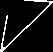
\includegraphics{figures/quad5.png}
	\end{subfigure}
	\caption{Quad candidates after segmentation}
	\label{fig:segmentationOutput}
\end{figure}

The next blob-filtering step is to filter out the false-positive contours.
These false hits can be caused by the light conditions or the scene around the marker.
For this purpose a simple metric is used to measure how likely a blob is to be a quad. 
This metric is the ratio of a blob's area and circumference. 
By experimentation this ratio for quads is found to be in the range of 10 and 50.
The contours with ratios outside these limits are discarded.

The segmentation processes output is available as a singe image with colour-coded\footnote{Gray level, to be exact} blobs or as a list of separate images each containing a quad candidate.
Figure \figref{segmentationOutput} shows an example for the output of the segmentation process.

%-----------------------------------------------------------------------------------------------
\subsection{Conditioning}
%-----------------------------------------------------------------------------------------------

Before running the line detection algorithms some conditioning steps are done in order to improve their effectiveness.
These processes are not uniform - every fitting method needs it's own.

The Hough transformation traditionally works best on thin lines.
The easiest way is to generate an edge image with high-pass filtering.
The OpenCV framework offers a wide variety of features for this task.
The best result are obtained by using the Canny edge detector.

The skeletoning detector does not need a conditioning step, as it performs the band thinning on it's own.

The methods based on image gradients and corner detection both require some level of smoothing on the picture.
In case of the corner detection the smoothing is useful for removing the false positive matches caused by the jagged edges, or in case os JPEG images the artefacts caused by the compression.
The gradient detector simply gives a more spread-out and easier to analyse result on a smoothly changing gradient than it would on strict edge.
The smoothing is also implemented using the OpenCV framework, which provides easy access to Gaussian filtering.
The OpenCV implementation is based on convolution with a configurable Gaussian kernel.
The kernel size and the deviation in $x$ and $y$ direction can be set.
The Gaussian kernel and the convolution itself is handled in th framework.

%-----------------------------------------------------------------------------------------------
\section{Line fitters}
%-----------------------------------------------------------------------------------------------



%-----------------------------------------------------------------------------------------------
\subsection{Hough transformation}
%-----------------------------------------------------------------------------------------------



%-----------------------------------------------------------------------------------------------
\subsection{Gradient detector}
%-----------------------------------------------------------------------------------------------



%-----------------------------------------------------------------------------------------------
\subsection{Corner detector}
%-----------------------------------------------------------------------------------------------



%-----------------------------------------------------------------------------------------------
\subsection{Skeletoning detector}
%-----------------------------------------------------------------------------------------------


